\section{Hyperbolic metric}
% \subsubsection{Mặt phẳng hyperbolic}
% Đối tượng nghiên cứu chính của chương này là \textit{mặt phẳng hyperbolic}
% \[\hh := \{z\in \C~|~\im(z) > 0\}.\] 
% Nhận thấy $\hh$ là nửa mặt phẳng trên, cũng là một tập con mở của mặt phẳng phức $\C$ với metric Euclid thông thường. Trên $\hh$, ta sẽ trang bị một metric, mà ta gọi là \textit{metric hyperbolic} nhằm giúp ta xác định \textit{khoảng cách, góc} giữa các đối tượng hình học trong $\hh$. Sau đó, ta tìm hiểu về các \textit{phép đẳng cự} trên $\hh$, đặc biệt là tìm hiểu \textit{tác động} của nhóm tuyến tính xạ ảnh đặc biệt $\PSL(2,\R)$ lên $\hh$.
\begin{defn}
    Mặt phẳng hyperbolic $\hh$ là tập con mở của mặt phẳng phức $\C$ bao gồm các điểm có phần ảo dương
    \[\hh=\{z\in \C: \im(z)>0\}\]
    trang bị tích vô hướng hyperbolic trên mỗi không gian vector tiếp xúc như sau. Với mọi điểm $z\in \hh$ và $u,v \in T_z\hh$ là các vector tiếp xúc tại $z$, tích vô hướng hyperbolic của $u$ và $v$ là 
    \[\left<u,v\right>_{hyp}=\dfrac{u\cdot v}{(\im(z))^2}\]
    trong đó $u\cdot v$ là tích vô hướng Euclid của $u$ và $v$.
\end{defn}
Tích vô hướng hyperbolic trên mỗi không gian tiếp xúc của mặt phẳng hyperbolic $\hh$ cho phép ta tính \textbf{độ dài hyperbolic} của các vector tiếp xúc. Cụ thể hơn, độ dài hyperbolic của một vector tiếp xúc $v\in T_z\hh$ là 
\[|v|_{hyp}=\sqrt{\left<u,v\right>_{hyp}} = \dfrac{|v|}{\im(z)}\]
trong đó $|v|$ là độ dài của $|v|$ đối với metric Euclid.

Tích vô hướng hyperbolic này cũng sinh ra các khái niệm vuông góc và góc hyperbolic.
\begin{prop}
    Cho $u,v \in T_z\hh$ là các vector tiếp xúc.
    \begin{enumerate}
        \item Hai vector $u,v$ vuông góc với nhau đối với tích vô hướng hyperbolic khi và chỉ khi chúng vuông góc với nhau đối với tích vô hướng Euclid.
        \item Giả sử $u$ và $v$ khác không. Khi đó, góc của $u$ và $v$ đối với tích vô hướng hyperbolic cũng là góc của $u$ và $v$ đối với tích vô hướng Euclid.
    \end{enumerate}
\end{prop}
\begin{proof}
    Với mọi $u,v \in T_z\hh$
    \begin{enumerate}
        \item Ta có $\left<u,v\right>_{hyp} = 0 \Leftrightarrow \dfrac{u\cdot v}{(\im(z))^2} = 0 \Leftrightarrow u\cdot v = 0$.
        
        Chứng tỏ $u \perp_{hyp}v $ khi và chỉ khi $u \perp_{Euclid} v$.
        \item Nếu $u,v$ khác không, khi đó góc giữa 2 vector $u,v$ thuộc $[0,\pi]$, cụ thể
        \[\cos\widehat{(u,v)}_{hyp} \defeq \dfrac{\left<u,v\right>_{hyp}}{|u|_{hyp}|v|_{hyp}} = \dfrac{\dfrac{u\cdot v}{(\im(z))^2}}{\dfrac{|u|}{\im(z)}\dfrac{|v|}{\im(z)}} = \dfrac{u\cdot v}{|u||v|} = \cos\widehat{(u,v)}_{Euclid}.\]
        Chứng tỏ góc của $u$ và $v$ đối với tích vô hướng hyperbolic cũng là góc của $u$ và $v$ đối với tích vô hướng Euclid.
    \end{enumerate}
\end{proof}

Nhắc lại rằng độ dài Euclid của một đường cong trơn từng khúc $\gamma: [a,b]\to \hh$ là 
\[l(\gamma) = \int_{a}^{b}|\gamma'(t)|dt.\]
Trong công thức trên, $|\gamma'(t)|$ là độ dài Euclid của vector tiếp xúc $\gamma'(t)$. Khi thay độ dài Euclid bởi độ dài hyperbolic, ta nhận được độ dài hyperbolic của một đường cong trơn từng khúc trong $\hh$.

\begin{defn}
    \textbf{Độ dài hyperbolic} của một đường cong trơn từng khúc $\gamma: [a,b]\to \hh$ là
    \[h(\gamma) = \int_a^b|\gamma'(t)|_{hyp}dt.\]
\end{defn}
\begin{exam*}
\begin{enumerate}
    \item Với mỗi $a>0$, xét đường tham số $\gamma_a: [\pi/3, 2\pi/3]\to \hh, t \mapsto ae^{it}$. Ta có
    \begin{itemize}
            \item Độ dài Euclid của $\gamma_a$ là
            \[l(\gamma_a) = \int_{\pi/3}^{2\pi/3}{|\gamma_a'(t)|dt} = \int_{\pi/3}^{2\pi/3}|aie^{it}|dt = a\pi/3.\]
            biến thiên, phụ thuộc vào giá trị của $a>0$. Đây chính là độ dài các cung tròn có số đo góc $\pi/3$ của các đường tròn bán kính $a$.
            \item Độ dài hyperbolic của $\gamma_a$ là
            \[h(\gamma_a) = \int_{\pi/3}^{2\pi/3}|\gamma_a'(t)|_{hyp}dt = \int_{\pi/3}^{2\pi/3}\dfrac{|\gamma_a'(t)|}{\im(\gamma_a(t))}dt = \int_{\pi/3}^{2\pi/3}{\dfrac{1}{\sin(t)}}dt = \ln{3}.\]
            không đổi với mọi giá trị $a>0$.
        \end{itemize}
        \begin{figure}[htp!]
            \centering
            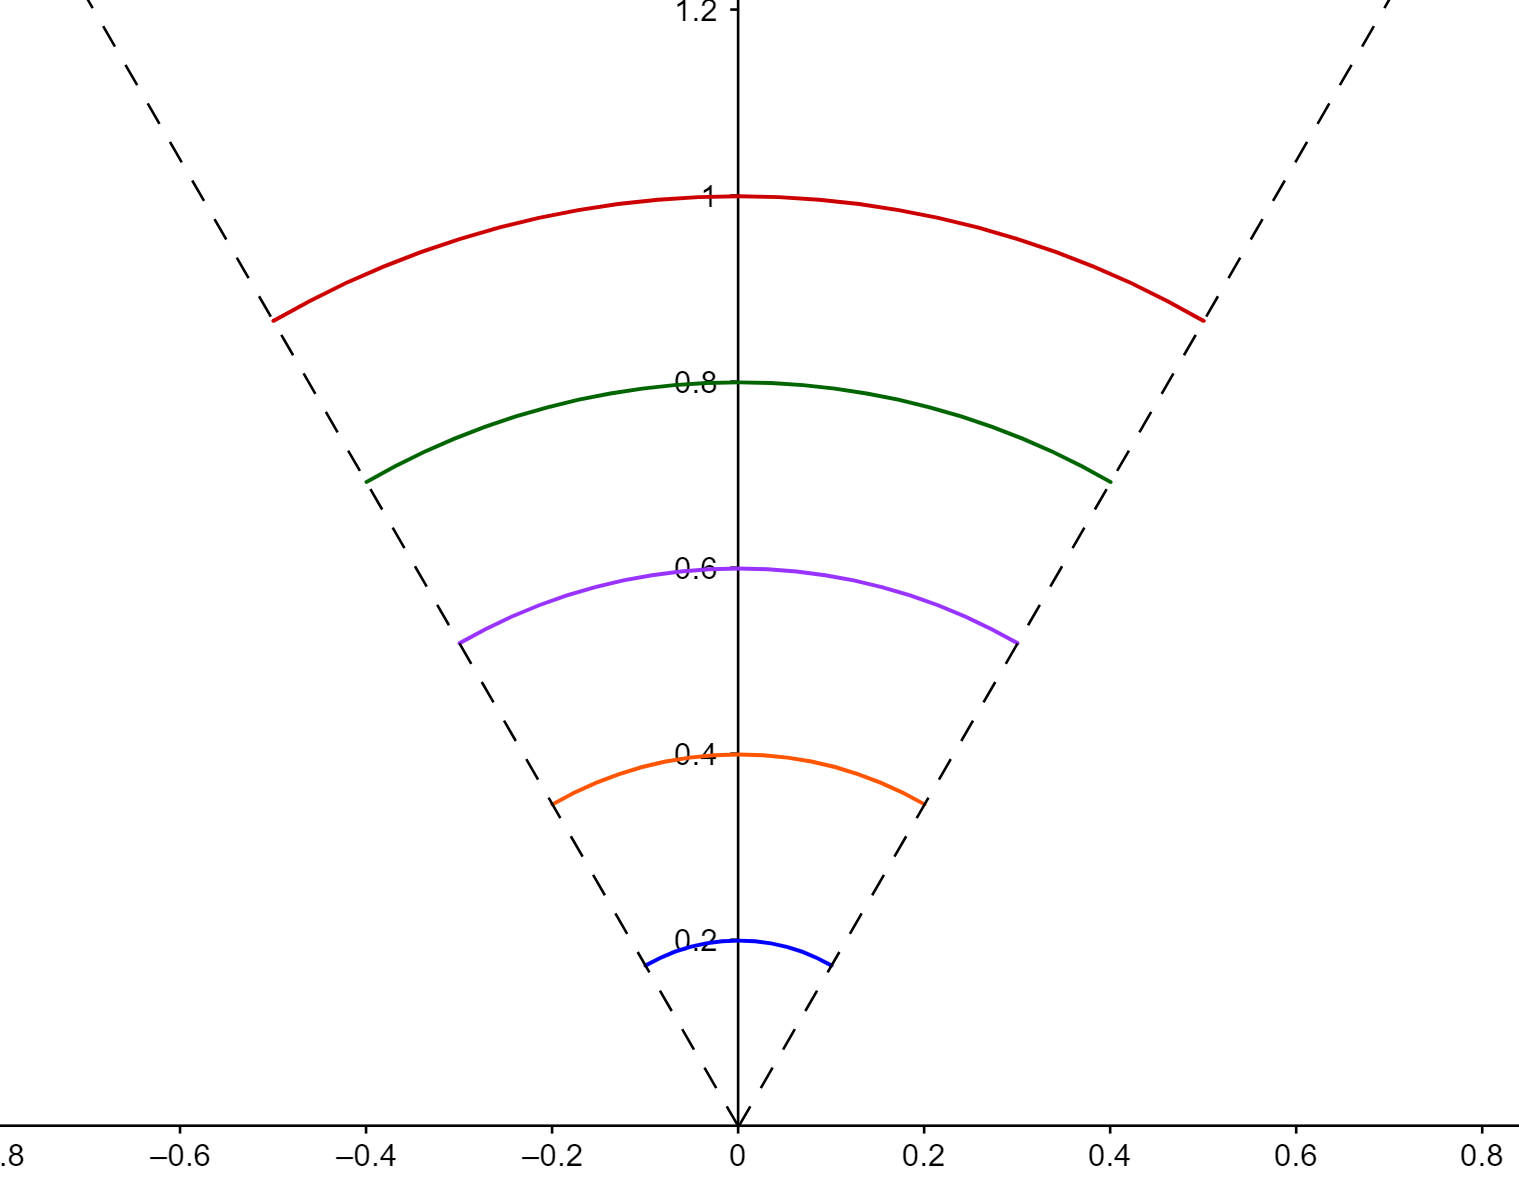
\includegraphics[width=0.4\linewidth]{images/Ex 2.1.4.3.png}
            % \caption{}
            % \label{fig:enter-label}
        \end{figure}


    \item Với mỗi số thực dương $b$, xét đường tham số $\gamma_b:[0,1]\to \hh$ cho bởi $\gamma_b(t) = t+ib$. Khi đó 
        \begin{itemize}
            \item Độ dài Euclid của $\gamma_b$ là
            \[l(\gamma_b) = \int_0^1{|\gamma'(t)|dt} = \int_0^1|1|dt = 1.\]
            không đổi với mọi $b>0$.
            \item Độ dài hyperbolic của $\gamma_b$ là
            \[h(\gamma_b) = \int_0^1|\gamma'(t)|_{hyp}dt = \int_0^1\dfrac{|\gamma'(t)|}{\im(\gamma(t))}dt = \int_0^1{\dfrac{1}{b}}dt = \dfrac{1}{b}.\]
            biến thiên, phụ thuộc vào giá trị của $b>0$. Khi $b \to \infty$ thì $h(\gamma_b) \to 0$. Ngược lại khi $b \to 0$ thì $h(\gamma_b) \to \infty$.
            \begin{figure}[htp!]
                \centering
                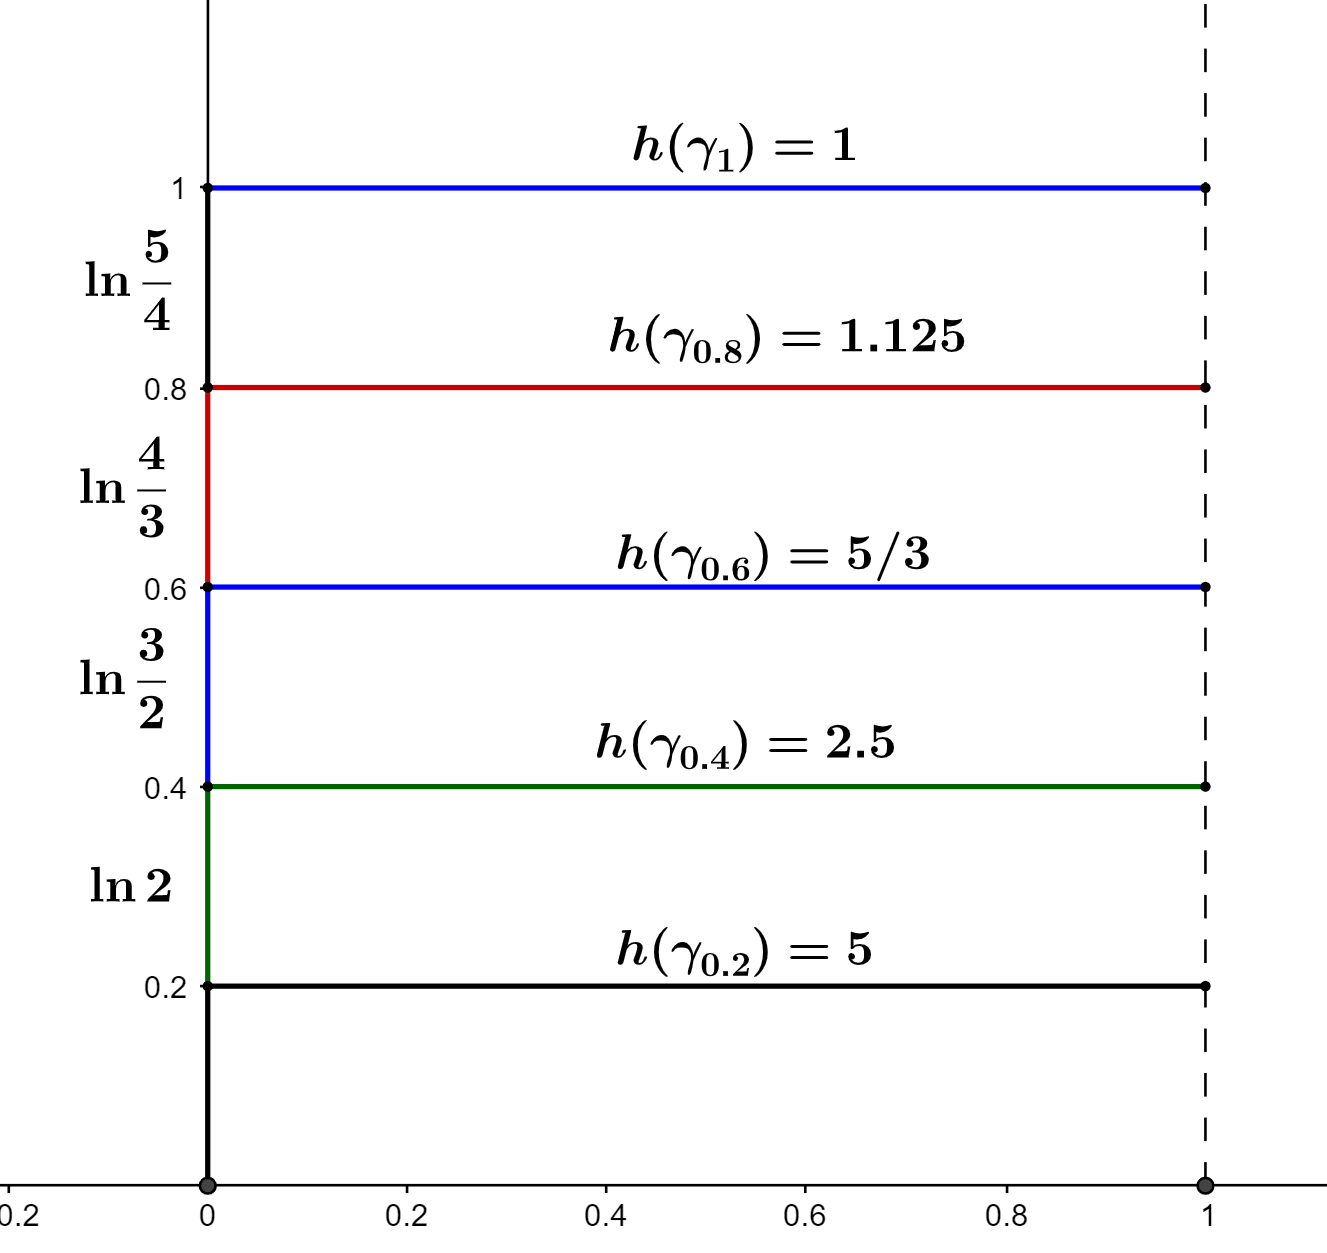
\includegraphics[width=0.5\linewidth]{images/it.png}
                % \caption{}
                % \label{fig:enter-label}
            \end{figure}
        \end{itemize}
    
        
\end{enumerate}
\end{exam*}

\begin{exam*}
    % \begin{enumerate}
        Cho $a<b$ là hai số thực dương. Khi đó độ dài hyperbolic của đường tham số $\gamma:[a,b]\to \hh$ cho bởi $\gamma(t) = it$ là
    \[h(\gamma) = \int_a^b|\gamma'(t)|_{hyp}dt = \int_a^b\dfrac{|\gamma'(t)|}{\im(\gamma(t))}dt = \int_a^b\dfrac{1}{t}dt = \ln{\dfrac{b}{a}}.\]
    %     \item Xét đường tham số $\alpha: [a,b] \to \hh,~t \mapsto ie^t$. Khi đó độ dài hyperbolic của $\gamma$ là
    %         \[h(\alpha) = \int_a^b|\alpha'(t)|_{hyp}dt = \int_a^b\dfrac{|\alpha'(t)|}{\im(\alpha(t))}dt = \int_a^b{\dfrac{e^t}{e^t}}dt = b-a.\]
            
    % \end{enumerate}
\end{exam*}
\begin{defn}
    Cho $z,w\in \hh$. \textbf{Khoảng cách hyperbolic} từ $z$ đến $w$ là 
    \[\rho(z,w) = \inf_{\gamma \in \Gamma[z,w]}{h(\gamma)}\]
    trong đó tập $\Gamma[z,w]$ là tập hợp các đường tham số trơn từng khúc từ $z$ đến $w$.
\end{defn}
Bên dưới, ta sẽ đưa ra công thức tường minh để tính khoảng cách hyperbolic giữa hai điểm bất kỳ trong $\hh$. Mệnh đề sau là vài tính chất đơn giản của hàm khoảng cách hyperbolic. Sau này, ta sẽ chỉ ra rằng hàm khoảng cách hyperbolic là một metric trên $\hh$, hơn nữa, topo sinh ra từ metric này chính là topo thông thường của $\hh$. 

\begin{prop}\label{prop 2.1.7}
    Cho $z,z_1,z_2,z_3 \in \hh$ là các điểm bất kỳ. Khi đó
    \begin{enumerate}
        \item $\rho(z,z) = 0,$
        \item $\rho(z_1,z_2) \geq 0,$
        \item $\rho(z_1,z_2) = \rho(z_2,z_1),$
        \item $\rho(z_1,z_2)+\rho(z_2,z_3) \geq \rho(z_1,z_3)$.
    \end{enumerate}
\end{prop}
\begin{proof}
    Đầu tiên ta chỉ ra $\rho$ là đối xứng, tức $\rho(z_1,z_2) = \rho(z_2,z_1)$ với mọi $z_1,z_2 \in \hh$. Thật vậy, 

        Lấy bất kỳ $\gamma:[a,b]\to \hh$ trong $\Gamma[z_1,z_2]$, cho hợp thành với song ánh khả vi sau 
    \[\tau: [a,b]\to [a,b],~t \mapsto (a+b-t).\]
    Khi đó $\sigma = \gamma\circ \tau:[a,b]\to \hh$ cũng là một hàm trơn từng khúc thoả mãn
    \[\sigma(a) = \gamma\circ \tau(a) = \gamma(b)=z_2,~\sigma(b) = \gamma\circ \tau(b) = \gamma(a)=z_1.\] 
    Chứng tỏ $\sigma \in \Gamma[z_2,z_1]$ và độ dài hyperbolic của $\sigma$ là
    \begin{align*}
        h(\sigma) = \int_{a}^{b}{\dfrac{\left|\sigma'(t)\right|}{\im(\sigma(t))}}dt = \int_{a}^{b}{\dfrac{\left|(\gamma\circ\tau)'(t)\right|}{\im((\gamma\circ\tau)(t))}}dt=\int_{a}^{b}{\dfrac{\left|\gamma'(\tau(t))\tau'(t)\right|}{\im(\gamma(\tau(t)))}}dt.
    \end{align*}
    Đặt $s = \tau(t) = a+b-t$ thì $ds = -dt$. Đổi cận $t=a$ thì $s = b$, $t=b$ thì $s=a$, kết hợp $\tau'(t) = -1$ ta được
    \begin{align*}
        h(\sigma) = -\int_{b}^{a}{\dfrac{\left|\gamma'(s)\right|}{\im(\gamma(s))}}ds = \int_{a}^{b}{\dfrac{\left|\gamma'(s)\right|}{\im(\gamma(s))}}ds = h(\gamma).
    \end{align*}
    Điều này chứng tỏ mỗi $\gamma \in \Gamma[z_1,z_2]$ sẽ tương ứng với $1-1$ với một $\sigma \in \Gamma[z_2,z_1]$, hơn nữa độ dài hyperbolic của hai đường này bằng nhau. 
    Dẫn đến 
    \[\left\{h(\gamma)~|~\gamma \in \Gamma[z_1,z_2]\} = \{h(\sigma)~|~\sigma \in \Gamma[z_2,z_1]\right\}.\]
    Lấy $\inf$ hai vế ta được 
    \[\rho(z_1,z_2) = \inf\{h(\gamma)~|~\gamma \in \Gamma[z_2,z_1]\} = \inf\{h(\sigma)~|~\sigma \in \Gamma[z_2,z_1]\} = \rho(z_2,z_1).\] 

    Tiếp theo ta chỉ ra $\rho$ thoả mãn bất đẳng thức tam giác.

    Thật vậy, giả sử $\gamma_{z_1,z_2}:[a,b]\to \hh$ và $\gamma_{z_2,z_3}:[b,c]\to \hh$ lần lượt thuộc $\Gamma[z_1,z_2]$ và $\Gamma[z_2,z_3]$. Khi đó $\gamma_{z_1,z_3}: [a,c] \to \hh$ cho bởi $\gamma_{z_1,z_3}(t) = \gamma_{z_1,z_2}(t)$ nếu $t\in[a,b]$ và $\gamma_{z_1,z_3}(t) = \gamma_{z_2,z_3}(t)$ nếu $t\in[b,c]$, là đường nối $z_1 \text{ tới }z_3$. Dẫn đến
    \[\rho(z_1,z_3) = \inf_{\gamma \in \Gamma[z_1,z_3]}\{h(\gamma)\} \leq h(\gamma_{z_1,z_3}) = h(\gamma_{z_1,z_2}) + h(\gamma_{z_2,z_3}).\]
    Lấy $\inf$ hai vế theo các đường cong trơn từng khúc nối $z_1 \text{ tới }z_2$ và nối $z_2 \text{ tới }z_3$ ta được
    \[\rho(z_1,z_3) \leq  \inf h(\gamma_{z_1,z_2}) + \inf h(\gamma_{z_2,z_3}) = \rho(z_1,z_2) + \rho(z_2,z_3).\]

    Cuối cùng ta kiểm tra tính xác định dương của $\rho$.

    Lấy $\gamma_0: [a,b] \to \hh, t \mapsto z$ là một đường cong trơn trên $\hh$ qua $z$. Ta có $\gamma_0'(t) = 0$ nên $h(\gamma_0) = 0 $. Vì vậy, $\rho(z,z) = 0$.

    Nếu $z_1 \neq z_2$, ta sẽ chỉ ra $\rho(z_1,z_2) >0$ sau.
\end{proof}
\begin{prop}\label{prop 2.1.8}
    Cho $a,b$ là hai số thực dương. Khoảng cách hyperbolic giữa các điểm $ia, ib$ là 
    \[\rho(ia,ib) = \left|\ln{\dfrac{b}{a}}\right|.\]
\end{prop}
\begin{proof}
    Xét trường hợp $0<a<b$.
    
    Xét đường cong $\gamma_0:[0,1] \to \hh,~t\mapsto x(t) + iy(t) = i(a+(b-a)t$ có đồ thị chính là đoạn thẳng Euclid trên trục ảo nối $ia$ với $ib$. Khi đó độ dài hyperbolic của $\gamma_0$ là 
    \[h(\gamma_0) = \int_{0}^{1}{\dfrac{\sqrt{(x'(t))^2+(y'(t))^2}}{y(t)}}dt = \int_{0}^{1}{\dfrac{b-a}{a+(b-a)t}}dt = \ln{|a+(b-a)t|~\bigg|_{0}^{1}} = \ln \dfrac{b}{a}.\]
    Lấy bất kì đường cong trơn từng khúc $\gamma: [0,1] \to \hh,~t \mapsto \gamma(t) = u(t) + i v(t)$ nối $ia$ và $ib$ (tức $\gamma(0)=u(0)+iv(0)=ia,~\gamma(1)=u(1)+iv(1)=ib$). Khi đó độ dài hyperbolic của $\gamma$ là
    \[h(\gamma) = \int_{0}^{1}{\dfrac{\sqrt{(u'(t))^2+(v'(t))^2}}{v(t)}}dt \geq \int_{0}^{1}{\dfrac{|v'(t)|}{v(t)}}dt \geq \int_{0}^{1}{\dfrac{v'(t)}{v(t)}}dt = \int_{a}^{b}{\dfrac{dv}{v}} = \ln\dfrac{b}{a } = h(\gamma_0)\cdot\]
    Chửng tỏ $\gamma_0$ chính là đường cong có độ dài hyperbolic ngắn nhất nối $ia$ và $ib$ trong $\hh$. Tức là $\rho(ia,ib) = \ln \dfrac{b}{a}\cdot$

    Tương tự cho trường hợp $a>b>0$ ta được $\rho(ia,ib) = \ln \dfrac{a}{b}\cdot$

    Tóm lại $\rho(ia,ib) = \left|\ln{\dfrac{b}{a}}\right|.$
\end{proof}
Để tính khoảng cách giữa hai điểm bất kỳ trong $\hh$, và xác định các trắc địa của $\hh$, ta sẽ sử dụng các đẳng cự của $\hh$.
\begin{defn}
    Một vi phôi $T:\hh \to \hh$ được gọi là một \textbf{đẳng cự} nếu với mọi $z\in \hh$ và mọi vector tiếp xúc $u,v \in T_z\hh$, ta có
    \[\left<DT_z(u),DT_z(v)\right>_{hyp} = \left<u,v\right>_{hyp}.\]
\end{defn}
\begin{prop}\label{prop 2.1.10}
    Cho $T$ là một phép đẳng cự của $\hh$.
    \begin{enumerate}
        \item Cho $\gamma$ là một đường tham số trơn từng khúc trong $\hh$. Khi đó $h(T(\gamma)) = h(\gamma)$.
        \item Cho $z,w$ là hai điểm của $\hh$. Khi đó $\rho(z,w) = \rho(T(z),T(w))$.
    \end{enumerate}
\end{prop}
\begin{proof}
    \begin{enumerate}
        \item Giả sử $\gamma: [a,b] \to \hh$ là một đường cong trơn từng khúc trong $\hh$. Khi đó
        \begin{align*}
            h(T(\gamma)) &= \int_a^b|(T\circ\gamma)'(t)|_{hyp}dt \\
            &= \int_a^b{\sqrt{\left<DT_{\gamma(t)}(\gamma'(t)),DT_{\gamma(t)}(\gamma'(t))\right>_{hyp}}}dt\\
            &= \int_a^b\sqrt{\left<\gamma'(t),\gamma'(t)\right>_{hyp}}dt\\
            &= \int_a^b|\gamma'(t)|_{hyp}dt\\
            &= h(\gamma).
        \end{align*}

        \item Với mọi $z,w \in \hh$, ta có
        \[\rho(z,w) = \inf_{\gamma\in \Gamma[z_1,z_2]}{h(\gamma)} = \inf_{\gamma\in \Gamma[z_1,z_2]}{h(T(\gamma))} = \inf_{\alpha  \in \Gamma[T(z),T(w)]}{h(\alpha)} = \rho(T(z),T(w))\]
    \end{enumerate}
\end{proof}
Tập hợp các phép đẳng cự của mặt phẳng hyperbolic lập thành một nhóm đối với phép toán hợp thành. Ta ký hiệu nhóm này là $\Isom(\hh)$ và gọi là nhóm các phép đẳng cự trên $\hh$.
\begin{prop}\label{prop 2.1.11}
    Cho $A = \matt \in \SL(2,\R)$. Xét các phép biến đổi xạ ảnh $T_A:P^1(\C) \to P^1(\C)$.
    \begin{enumerate}
        \item Với mọi $z\in \hh, T_A(z) \in \hh$. Hơn nữa
        \[T_A(z) = \dfrac{az+b}{cz+d}.\]
        \item Ánh xạ hạn chế $T_A: \hh \to \hh$ là một vi phôi.
    \end{enumerate}
\end{prop}
\begin{proof}
    \begin{enumerate}
        \item Với mọi $z\in \hh$, ta có 
            \begin{align*}
            \im(T_A(z)) &= \dfrac{1}{2i}\left(T_A(z) - \overline{T_A(z)}\right)\\
            &= \dfrac{1}{2i}\left(\dfrac{az+b}{cz+d} - \dfrac{a\overline{z}+b}{c\overline{z}+d}\right) \quad (\text{do } a,b,c,d \in \R)\\
            &= \dfrac{1}{2i}\left(\dfrac{(ad-bc)(z-\overline{z})}{|cz+d|^2}\right)\\
            &= \dfrac{\im(z)}{|cz+d|^2} > 0\quad(\text{do } z \in \hh \text{ nên } \im(z) >0).
            \end{align*}
            Chứng tỏ $T_A(z) \in \hh$ với mọi $z\in \hh$.

            \item Ta có $T_A$ là một song ánh khả vi liên tục và nghịch ảnh của nó $T_A^{-1}(z) = \dfrac{dz-b}{-cz+a}$ cũng thuộc $\PSL(2,\R)$ và cũng khả vi liên tục. Do đó $T_A$ là một vi phôi trên $\hh$.
            % \[T_A'(z) = \dfrac{ad-bc}{(cz+d)^2} = \dfrac{1}{(cz+d)^2}.\]
    \end{enumerate}
\end{proof}

Ta nói ánh xạ hạn chế $T_A: \hh \to \hh$ là phép biến đổi của mặt phẳng hyperbolic sinh bởi ma trận $A$.
\begin{prop}\label{prop 2.2.12}
    Cho $A\in \SL(2,\R)$. Khi đó, phép biến đổi $T_A:\hh \to \hh$ của mặt phẳng hyperbolic sinh ra bởi ma trận $A$ là một đẳng cự.
\end{prop}
\begin{proof}
    Giả sử $A = \matt$.  Khi đó phép biến đổi của mặt phẳng hyperbolic sinh bởi $A$ là $T_A(z) = \dfrac{az+b}{cz+d}$. Với mọi $z\in \hh$ và với mọi $u,v \in T_z\hh$ ta có
    \begin{align*}
        \left<(DT_A)_z(u),(DT_A)_z(v)\right>_{hyp} 
        &= \left<\dfrac{1}{(cz+d)^2}(u),\dfrac{1}{(cz+d)^2}(v)\right>_{hyp} \\
        & = \dfrac{\dfrac{1}{(cz+d)^2}(u) \cdot \dfrac{1}{(cz+d)^2}(v)}{\im^2(T_A(z))}\\
        &= \dfrac{\left|\dfrac{1}{(cz+d)^2}\right|u\cdot v}{\left(\dfrac{\im(z)}{|cz+d|^2}\right)}\\
        &= \dfrac{u\cdot v}{\im^2(z)}\\
        &= \left<u,v\right>_{hyp}.
    \end{align*}
    Chứng tỏ $T_A$ là một đẳng cự trên $\hh$.
\end{proof}

Ta nhận được đồng cấu nhóm 
\begin{equation}\label{equ 2.1.1}
\SL(2,\R) \to \Isom(\hh),\quad A \mapsto T_A.
\end{equation}
\begin{prop}\label{prop 2.1.13}
    Hạt nhân của đồng cấu nhóm \ref{equ 2.1.1} là nhóm con của $\SL(2,\R)$ bao gồm hai ma trận $\begin{bmatrix}
        1 & 0\\
        0 & 1
    \end{bmatrix}, \begin{bmatrix}
        -1 & 0\\
        0 & -1
    \end{bmatrix}$. Do đó đồng cấu nhóm \ref{equ 2.1.1} cảm sinh đơn cấu $\PSL(2,\R) \to \Isom(\hh)$. 
\end{prop}
\begin{proof}
    Đồng cấu nhóm $\phi: \SL(2,\R) \to \Isom(\hh),A \mapsto T_A$ có hạt nhân \[\ker(\phi) = \{A \in \SL(2,\R): T_A = \Id\}\]

    Để $A  = \matt \in \ker(\phi)$ thì $z = T_A(z) = \dfrac{az+b}{cz+d}$  với mọi $z\in \hh$.
    Đồng nghĩa với việc phương trình $cz^2+(d-a)z+b = 0$ có vô số nghiệm. Điều này xảy ra khi và chỉ khi $c=d-a=b=0$. Kết hợp $ad-bc=1$ ta thu được $b=c=0, a=d=\pm 1$. Do đó $\ker(\phi)= \{\pm I_2\}$, với $I_2$ là ma trận đơn vị cỡ 2.

    Khi đó $\PSL(2,\R) = \SL(2,\R)/\ker(\phi) \cong \im(\phi) \leq \Isom(\hh)$ cảm sinh một đơn cấu $\PSL(2,\R) \to \Isom(\hh)$.
\end{proof}
Sử dụng đơn cấu $\PSL(2,\R) \to \Isom(\hh)$ trong mệnh đề trên, ta thường coi $\PSL(2,\R)$ là một nhóm con của $\Isom(\hh)$.
% \begin{exam*}
%     Tính khoảng cách hyperbolic giữa hai điểm $z=1+i$ và $w=-3+4i$ trong $\hh$. Xác định các đường tham số $\gamma$ nối $z$ đến $w$ sao cho $h(\gamma) =\rho(z,w)$.

%     Dựa vào mệnh đề \ref{prop 2.1.8} và mệnh đề \ref{prop 2.1.10}, ta sẽ tìm một đẳng cự $T(z) = \dfrac{az+b}{cz+d}$ gửi hai điểm $1+i$ và $-3+4i$ thành hai điểm có phần ảo dương trên trục ảo.

%     Ta tìm $a,b,c,d \in \R$ thoả mãn $ad-bc = 1$ và $T(1+i) = i$ và $\re(T(w)) = 0$. 
%     \begin{itemize}
%         \item  $T(i+1) = i \Leftrightarrow \dfrac{a(1+i)+b}{c(1+i)+d}=i \Leftrightarrow (a+b)+ia = -c +(c+d)i \Leftrightarrow a+b = -c,~a = c+d$.

%         \item $\re(T(w)) = 0 \Leftrightarrow \dfrac{1}{2}\left(\dfrac{aw+b}{cw+d}+\dfrac{a\overline{w}+b}{c\overline{w}+d}\right) = 0 \Leftrightarrow ac|w|^2+(ad+bc)\re(w)+bd = 0\Leftrightarrow 25ac-3(ad+bc) +bd = 0$.
%         \item Suy ra $25ac -3a(a-c)-3c(-c-a) +(-c-a)(a-c) = 0 \Leftrightarrow 4c^2+31ca-4a^2 = 0 \Leftrightarrow c = \dfrac{-31\pm 5\sqrt{41}}{8}a$. Ta chọn $c = \dfrac{-31+ 5\sqrt{41}}{8}a$

%         Kết hợp $1 = ad-bc = a(a-c)-(-c-a)c = a^2+c^2$, ta được $a= \dfrac{8}{\sqrt{2050-310\sqrt{41}}}$. 
        
%         Dẫn đến $c = \dfrac{-31+5\sqrt{41}}{\sqrt{2050-310\sqrt{41}}}$. Suy ra $b = \dfrac{-23-5\sqrt{41}}{\sqrt{2050-310\sqrt{41}}},~d = \dfrac{39-5\sqrt{41}}{\sqrt{2050-310\sqrt{41}}}.$

%         Do đó $T(w) = i\im(T(w)) = i \dfrac{1}{|cw+d|^2} = i\dfrac{2050-310\sqrt{41}}{38792-6040\sqrt{41}}.$

%         Khi đó $\rho(z,w) = \rho(T(z),T(w)) = \rho\left(i,i\dfrac{2050-310\sqrt{41}}{38792-6040\sqrt{41}}\right) = \ln{\dfrac{38792-6040\sqrt{41}}{2050-310\sqrt{41}}}.$

%         Do đó ta chọn được $\gamma: [1, \im(T(w))] \to \hh, ~t \to T^{-1}(it)$ là đường cong trơn qua $z,w$ thoả mãn $h(\gamma) = \rho(z,w)$.
%     \end{itemize}
    
% \end{exam*}
\begin{exam*}
    Tính khoảng cách hyperbolic giữa hai điểm $z=1+i$ và $w=-2+2i$ trong $\hh$. Xác định các đường tham số $\gamma$ nối $z$ đến $w$ sao cho $h(\gamma) =\rho(z,w)$.

    Dựa vào mệnh đề \ref{prop 2.1.8} và mệnh đề \ref{prop 2.1.10}, ta sẽ tìm một đẳng cự $T(z) = \dfrac{az+b}{cz+d}$ gửi hai điểm $1+i$ và $-2+2i$ thành hai điểm có phần ảo dương trên trục ảo.

    Ta tìm $a,b,c,d \in \R$ thoả mãn $ad-bc = 1$ và $T(1+i) = i$ và $\re(T(w)) = 0$. 
    \begin{itemize}
        \item  $T(i+1) = i \Leftrightarrow \dfrac{a(1+i)+b}{c(1+i)+d}=i \Leftrightarrow (a+b)+ia = -c +(c+d)i \Leftrightarrow b = -c-a,~d = a -c$.

        \item $\re(T(w)) = 0 \Leftrightarrow \dfrac{1}{2}\left(\dfrac{aw+b}{cw+d}+\dfrac{a\overline{w}+b}{c\overline{w}+d}\right) = 0 \Leftrightarrow ac|w|^2+(ad+bc)\re(w)+bd = 0$.
        \item Suy ra $8ac -2a(a-c)-2c(-c-a) +(-c-a)(a-c) = 0 \Leftrightarrow c^2+4ca-a^2 = 0 \Leftrightarrow c = (-2\pm \sqrt{5})a$. Ta chọn $c = (-2+ \sqrt{5})a$. 

        Kết hợp $1 = ad-bc = a(a-c)-(-c-a)c = a^2+c^2$, ta được $a^2=\dfrac{1}{10-4\sqrt{5}}$. 
        
        Chọn $a = \dfrac{1}{\sqrt{10-4\sqrt{5}}}$. Suy ra $c = \dfrac{-2+\sqrt{5}}{\sqrt{10-4\sqrt{5}}}, b = \dfrac{1-\sqrt{5}}{\sqrt{10-4\sqrt{5}}},~d = \dfrac{3-\sqrt{5}}{\sqrt{10-4\sqrt{5}}}.$

        Do đó $T(w) = i\im(T(w)) = i \dfrac{\im(w)}{|cw+d|^2} = i\dfrac{7+3\sqrt{5}}{2}.$

        Khi đó $\rho(z,w) = \rho(T(z),T(w)) = \rho\left(i,i\dfrac{7+3\sqrt{5}}{2}\right) = \ln{\dfrac{7+3\sqrt{5}}{2}}.$

        Do đó ta chọn được $\gamma: [1, \im(T(w))] \to \hh, ~t \to T^{-1}(it)$ là đường cong trơn qua $z,w$ thoả mãn $h(\gamma) = \rho(z,w)$.
    \end{itemize}
    
\end{exam*}